\subsection{Use-Case}

% Outline for bug reports:
%  - Describe each system under test
%  - Describe bugs found
%  - Lessons learned from finding bugs
Here we present a hypothetical use-case from two perspectives
for correspondence checking and \simulator{}.

\noindent{\bf Network Operator.} An enterprise network
operator pays a third-party SDN provider to virtualize their network
and run it in the cloud. The network operator receives a complaint
from an internal team that two servers cannot reach other, and 
verifies the reachablility problem with {\tt ping}. Unsure
whether the problem is in her ACL/routing rules 
or in the underlying SDN platform, the
operator runs correspondence checking on a snapshot of the network state. She
finds that there is an inconsistency between her policy and the network state, 
and proceeds to call up the third-party SDN provider to complain
about the problem.

\noindent{\bf SDN Developer.} A developer at the third-party SDN
company receives the customer's trouble-ticket and begins to investigate the
problem. The developer examines the system logs and sees a
long list of link status events, control server reboots, VM migration events,
and other diagnostic information. These events are numerous (the
datacenter contains 8,000 switches and more than 100,000 hosts) and
interleaved, so the developer is unsure what caused the problem.
The developer feeds a snapshot of the network from before the
trouble-ticket was issued into the simulator, and
begins replaying the execution of the system. The developer runs
correspondence checking and finds a substantial list of policy-violations,
manifesting as loops, blackholes, and other problems.
The developer excludes all external events
unrelated to the two disconnected hosts. As the developer is stepping through the execution, he periodically
runs correspondence checking and tracks the policy-violations over time. He
finds that most violations resolve within a short time. However, he
eventually encounters a blackhole that lasts a considerable time. The
developer backs up the execution to the point when the blackhole begins, and
observes a switch failure followed directly by a reboot of the switch's parent
controller. A correspondence check between the intermediate layers of the SDN
stack indicate that the problem is present in the
physical view, but is not manifest in the virtualization layer. The developer adds log statements to the platform's failover
logic, and re-runs the execution. The developer eventually verifies that the
controller pushed a routing change to the failed switch's neighbors, but did
not update the platform's representation of the network state. Upon closer
examination, the developer finds that the new parent controller for that
portion of the network assumed that the platform's
representation of network state was up-to-date. As such, the partially installed flow entries remained
in the neighboring switches, resulting in the blackhole. The developer fixes
the platform's recovery code, adds this case to the platform's integration
test suite, and pushes the change to production. 

\subsection{Overhead}

\noindent{\bf Simulator Scalability.} Will a single machine be able to 
simulate large networks quickly enough for interactive use? In
Figure~\ref{fig:scalability} we depict the runtime for control processing vs.
number of simulated switches. We find the foobar. Our simulator keeled over at
X switches because of bottleneck Y.

\begin{figure}[t]
    %\hspace{-10pt}
    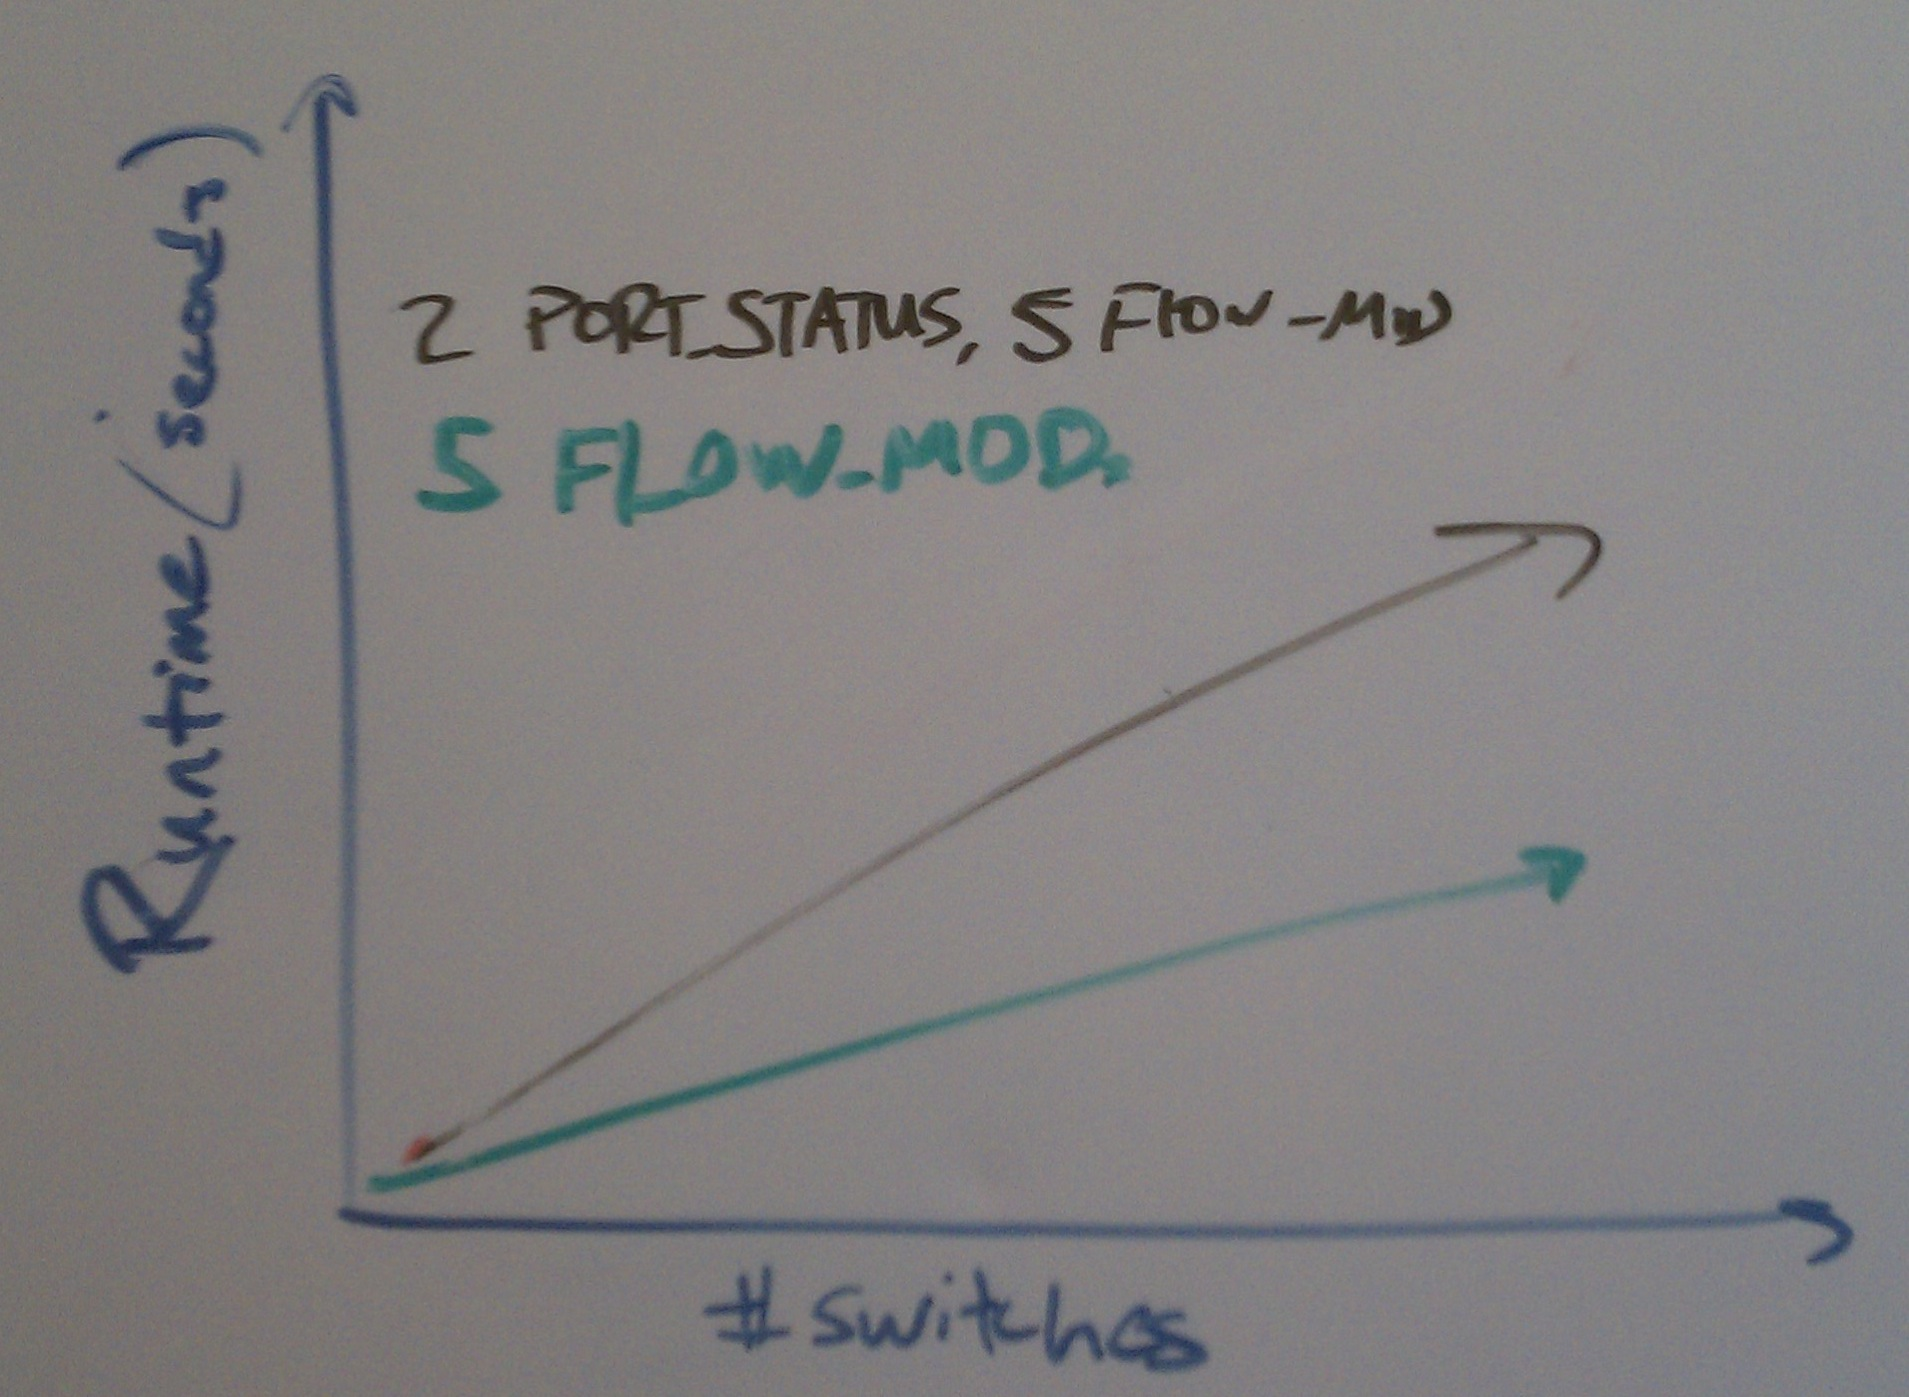
\includegraphics[width=3.25in]{../graphs/mock_simulator_scalability.jpg}
    \caption[]{\label{fig:scalability} Our beautfiful scalability graph}
\end{figure}

\noindent{\bf Record and Replay Overhead.} In contrast to general record-and-replay
mechanisms, the amount of recorded state needed for
high-fidelity replay is tractable. With proactive flow installation, 
updates are pushed to routing tables over a relatively long time scale; periodic
FIB snapshots along with a log of link state events, control server
downtime, and host mobility information suffice for our purposes. As a point of reference, the Cisco 7000 
core switch model supports a maximum of 128K MAC entries and
128K ACL entries~\cite{cisco7000}. Assuming 36 bytes per flow entry,
(larger than the OpenFlow 13-tuple), each FIB will contain a maximum of 9216
bytes, uncompressed. A datacenter of 100,000
hosts includes roughly 8,000
switches~\cite{Al-Fares:2008:SCD:1402958.1402967}.
Therefore a snapshot of the FIBs of the entire network takes up roughly 74 MB.
The VL2 paper reports 36M network error events over one year over 8
datacenters, which implies 8.5 error events per minute per
datacenter~\cite{Greenberg:2009:VSF:1592568.1592576}.
Suppose we took a snapshot of the FIBs in the network every second. 
Then we would need to store roughly 4GB, uncompressed, per minute, a relatively small growth 
rate for datacenter logs. This information, in addition to a log of host
mobility events (\eg{} VM migrations) will suffice for our purposes. Note that this is a conservative overestimate.
%To account for host mobility, assume that each server hosts 10 VMs,
%and 1\% of VMs are created, suspended, or migrated every minute. Then 10,000 host mobility events must be
%logged per minute, also a reasonable storage cost. \colin{get real numbers}

%As a point of reference, border routers' working RIB size is
%$\textasciitilde$130MB~\cite{Karpilovsky:2006:UFR:1368436.1368439}.

\noindent{\bf Correspondence Checking Runtime.} Computing the propagation
graph for correspondence checking is equivalent to enumerating
all possible paths in the network, which scales with the diameter
of the network and the number of routing entries per switch.
The propagation graph for each host can be
computed in parallel however, so the computation is bottlenecked by the serial runtime
of computing a single host's propagation graph.

We show the serial runtime of correspondence checking in 
Figure~\ref{fig:hsa_runtime}. For this analysis we generated fat tree topologies
between 2 and 48 pods wide, with pre-installed PORTLAND~\cite{NiranjanMysore:2009:PSF:1592568.1592575}
routing tables in each switch. Each data point is the minimum of three
runs on a single Intel Xeon 2.80GHz core. Note that the number of PORTLAND routing entries per switch scales with the number
of pods in the fat-tree. We excluded the time to convert
flow tables to HSA transfer functions, since transfer functions can be maintained
offline.

As the figure depicts, even for large networks
(27,648 hosts) the serial runtime of correspondence checking is reasonable for
interactive use. The number of serial tasks to be executed
is the number of hosts in the network squared, disregarding ECMP load balancing.

\begin{figure}[t]
    %\hspace{-10pt}
    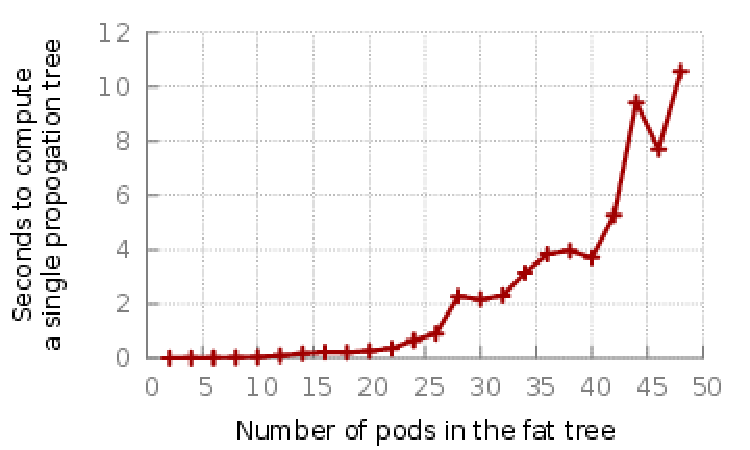
\includegraphics[width=3.25in]{../graphs/hsa_overhead_graph/graph.pdf}
    \caption[]{\label{fig:hsa_runtime} Serial runtime of correspondence
    checking on PORTLAND fat tree networks. Each datapoint consists of
    $x^3/4$ hosts and $5x^2/4$ switches (\eg{} 48 pods means 27,468 hosts
    attached to 2,880 switches)}
\end{figure}

\subsection{Replay fidelity}

If our simulated model of the network is not sufficiently complex, it may not
be able to reproduce error conditions observed in production. Conversely,
resolving bugs observed in a simulated environment may not ensure
correct behavior of the production network. In future work, we hope to verify
the fidelity of \simulator{} by collaborating with industry partners to
reproduce bugs observed in practice. In addition, we
plan to gather error logs by deploying our own applications in Google's
datacenter networking research cluster~\cite{DNRC}.

Finally, note that our correspondence checking algorithm can not verify 
time-dependent policies such as ``No link should be congested more than 1\% of the
time'', or ``No server should receive more than 500MB/s of external traffic''.
In future work we will extend our correspondence checking algorithm to
account for this class of policies.
